\documentclass[tikz,border=13pt]{standalone}
\usepackage[T1]{fontenc}
\begin{document}
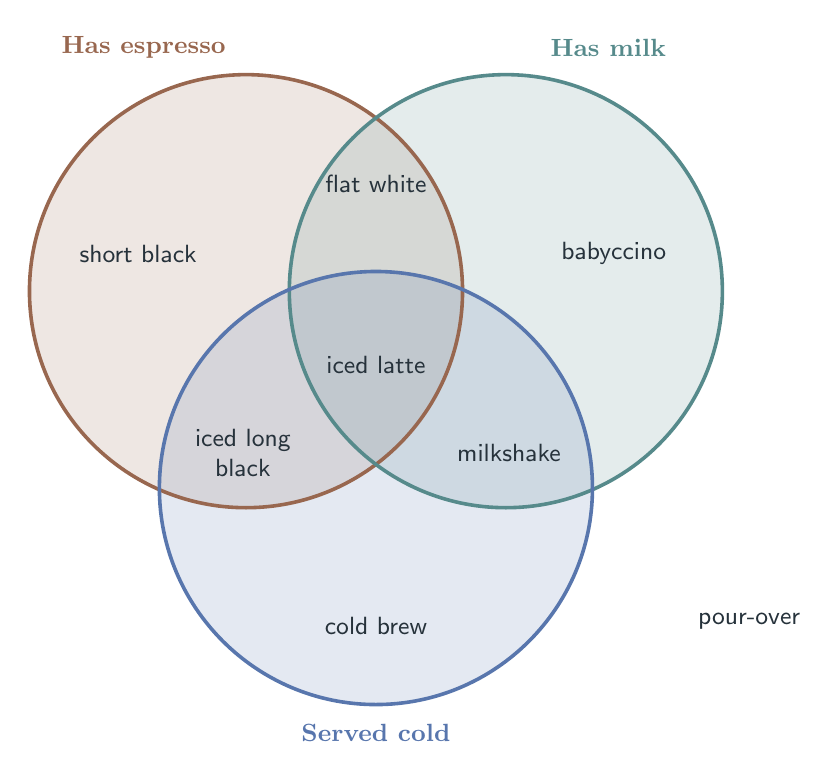
\begin{tikzpicture}[font=\sffamily]
  \definecolor{espresso}{HTML}{98674F}
  \definecolor{milk}{HTML}{568A8B}
  \definecolor{cold}{HTML}{5876AD}
  \definecolor{ink}{HTML}{26323B}
  \def\r{2.75}
  % Transparent fills leave every intersection visible.
  \fill[espresso,opacity=.16] (-1.65,.95) circle (\r);
  \fill[milk,opacity=.16] (1.65,.95) circle (\r);
  \fill[cold,opacity=.16] (0,-1.55) circle (\r);
  \draw[espresso,line width=1.3pt] (-1.65,.95) circle (\r);
  \draw[milk,line width=1.3pt] (1.65,.95) circle (\r);
  \draw[cold,line width=1.3pt] (0,-1.55) circle (\r);

  \node[font=\bfseries\small,text=espresso] at (-2.95,4.04) {Has espresso};
  \node[font=\bfseries\small,text=milk] at (2.95,4.04) {Has milk};
  \node[font=\bfseries\small,text=cold] at (0,-4.66) {Served cold};

  \tikzset{drink/.style={text=ink,font=\sffamily\small,align=center}}
  \node[drink] at (-3.02,1.43) {short black};
  \node[drink] at (3.02,1.43) {babyccino};
  \node[drink] at (0,2.31) {flat white};
  \node[drink] at (-1.69,-1.10) {iced long\\black};
  \node[drink] at (1.69,-1.10) {milkshake};
  \node[drink] at (0,.02) {iced latte};
  \node[drink] at (0,-3.30) {cold brew};
  \node[drink] at (4.74,-3.24) {pour-over};
\end{tikzpicture}
\end{document}
